\documentclass[letterpaper,superscriptaddress,aps,pra,nolongbibliography,nobibnotes,twocolumn,showpacs,groupedaddress,floatfix]{revtex4} % Packages and command definitions {{{
\usepackage{graphicx}
\graphicspath{{images/},{figures/},{eps/}}

% \ifpdf
% \pdfpagewidth=8.5 true in
% \pdfpageheight=11 true in
% \fi
% \usepackage[utf8]{inputenc}

\renewcommand{\arraystretch}{0}
\usepackage{amsmath, amsthm, amssymb}
\newcommand{\rmi}{\mathrm{i}}
\newcommand{\rme}{\mathrm{e}}
\newcommand{\eref}[1]{eq.~(\ref{#1})} \newcommand{\sref}[1]{sec.~\ref{#1}}
\newcommand{\rmd}{\mathrm{d}}
\newcommand{\fref}[1]{fig.~\ref{#1}}  \newcommand{\tref}[1]{table~\ref{#1}}
\newcommand{\Eref}[1]{Eq.~(\ref{#1})} \newcommand{\Sref}[1]{Sec.~\ref{#1}}
\newcommand{\Fref}[1]{Fig.~\ref{#1}}  \newcommand{\Tref}[1]{Table~\ref{#1}}
\newcommand{\tr}{\mathop{\mathrm{tr}}\nolimits}
\newtheorem{theorem}{Theorem}
\newcommand{\pder}[2]{\frac{\partial#1}{\partial#2}}

\def\>{\rangle} \def\<{\langle}
\def\q{{\textrm{q} }}
\def\env{{\textrm{env} }}
\def\cen{{\textrm{cen } }}
\def\inte{{\textrm{int } }}
\def\H{{\textrm{H}} }
\newcommand{\mcH}{\mathcal{H}}
\newcommand{\mcP}{\mathcal{P}}

% }}}
\begin{document}
% Title, abstract, authors {{{ WEEEEEE
\title{The ABC}
\newcommand{\unam}{Universidad Nacional Aut\'onoma de M\'exico, M\'exico}

\renewcommand{\paragraph}[1]{{\it #1.--}}


\newcommand{\ifunam}{Instituto de F\'{\i}sica, \unam}
\newcommand{\ifunamint}{\affiliation{Instituto de F\'{\i}´ısica, Universidad Nacional Aut\'onoma de M\'exico, 01000 M\'exico D.F., Mexico}}

\newcommand{\cic}{\affiliation{Centro Internacional de Ciencias A. C., Avenida Universidad s/n, 62131 Cuernavaca,
Mexico}}
\newcommand{\icf}{\affiliation{Instituto de Ciencias F\'{\i}sicas, 
Universidad Nacional Aut\'onoma de M\'exico, Avenida Universidad s/n, 62210 Cuernavaca, Morelos, Mexico}}
\newcommand{\uPotsdam}{\affiliation{Institut f\"ur Physik und Astronomie, University of Potsdam, 14476 Potsdam, Germany}}
\newcommand{\uSatya}{\affiliation{Laboratoire de Physique Th\'eorique et Mod\`eles Statistiques (UMR 8626 du CNRS), 
Universit\'e Paris-Sud, B\^atiment 100, 91405 Orsay Cedex, France}}


\author{Carlos Pineda} \email{carlospgmat03@gmail.com} \ifunamint
% \author{Satya N. Majumdar} \uSatya
\author{Thomas H. Seligman} \icf \cic
% \author{Celine} \uSatya
 



\begin{abstract}
Abstract
\end{abstract}
\pacs{05.30.Ch,03.65.-w,03.65.Yz}
% 05.30.Ch	Quantum ensemble theory
% 03.65.-w	Quantum mechanics [see also 03.67.-a Quantum information;
% 03.65.Yz	Decoherence; open systems; quantum statistical methods 
\maketitle
% }}}

\section{Introduction} %{{{ WEEE
We are interested in a tripartite Hilbert space 
\begin{equation}
\mcH = \mcH_A \otimes \mcH_B \otimes \mcH_C 
\label{}
\end{equation}
in which $\mcH_C$ plays the roll of a central system,
$\mcH_B$ is a near environment with which the central 
system interacts, and $\mcH_A$ is a far environment with which 
the central system does not interact, but the near environment does. 
We shall denote $N_i = \dim \mcH_i$, $i=A,B,C$, the dimensions 
of the Hilbert spaces. We shall often have the short $N$ for $(N_A,N_B,N_C)$.

We consider the following  Hamiltonian, which we call the ABC Hamiltonian, in
which the indices indicate in which Hilbert spaces they act nontrivially. 
The Hamiltonian of the environment is
\begin{equation}
H_\env= \cos \theta(H_A + H_B) +  \gamma \sin \theta  V_{AB} 
\label{}
\end{equation}
{\bf porque no tengo a la gama multiplicando al primer termino?}
Notices that $\theta$ helps modulate if we have an single big environment, 
or an environment composed by to parts. 
The Hamiltonian of the central system is simply 
\begin{equation}
H_\cen= H_C 
\label{}
\end{equation}
and the interaction is 
\begin{equation}
H_\inte= V_{BC}.
\label{}
\end{equation}
The total Hamiltonian is simply 
\begin{equation}
H = H_\env+ H_\cen +\lambda H_\inte.
\label{}
\end{equation}
Notice that aside from the dimension of the parts, we have three parameters. 
$\theta$ was already discussed, whereas $\gamma$ modulates the interaction 
between the near and far environment and 
$\lambda$ controls the interactions of the central system and the near environment.


\begin{figure} % Figure  Entropy distribution for given purity  {{{
\begin{center}
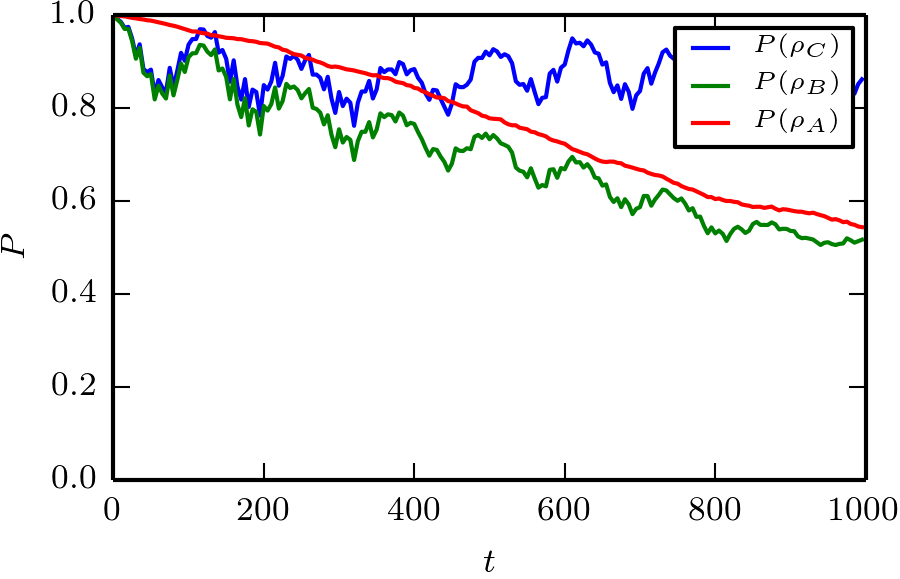
\includegraphics{no_explanation_1}
\end{center}
\caption{\label{fig:entropy:for:purity} (Color online)  Example for
$N=(20,4,2)$, $\theta = \pi/2$, $\gamma=\lambda=0.1$.}
\end{figure} % }}}



% }}}
% {{{ Acknowledgments. 
{\em Acknowledgments--}
% \author{Satya N. Majumdar} \uSatya
We thank La Rana Rene for very stimulating discussions at the onset of this project.
Support by the  projects CONACyT 153190 and
UNAM-PAPIIT IA101713 and UNAM-PAPIIT IG101113 are acknowledged.
% }}}
% \section*{References} % {{{ 
\bibliographystyle{unsrt}
\bibliography{paperdef,mibibliografia,library}
% }}}
\appendix
\section{An appendix} % {{{ 
Here an appendix
% }}}
\end{document}
